\documentclass[aspectratio=169]{beamer}

\usepackage{xmpmulti,multimedia,xspace}
\usepackage[latin1]{inputenc}
\usepackage{tikz}
\usetikzlibrary{shadows}
\usepackage{graphicx}
\graphicspath{{./img/} }


%\usetheme{Berlin}
\usetheme{AnnArbor}

\setbeamercovered{invisible}
\setbeamersize{text margin left=7.5mm}
\setbeamersize{text margin right=7.5mm}

%==============================================================================

\newcommand{\pitem}{\pause \item}

\begin{document}
\title{C Programming Tools: Part 3}
\subtitle{Building your own Tools}
\institute[Imperial]{Dept of Computing, \\
	Imperial College London}
\date{June 2019}
\newcommand\RBox[1]{%
%  \tikz\node[draw,rounded corners,align=center,] {#1};%
  \tikz\node[draw,rounded corners,align=center,double copy shadow={opacity=0.3,shadow xshift=1ex,shadow yshift=-0.5ex,left color = brown!40,right color = magenta!80},left color=blue!50,right color=yellow!50 ] {#1};%
}  
\setbeamerfont{author in head/foot}{size={\fontsize{3pt}{4pt}\selectfont}}
\author[Duncan White]
{%
   \texorpdfstring{
        \begin{columns}
            \column{.8\linewidth}
            \centering
            \RBox{Duncan C. White\\
            \href{mailto:d.white@imperial.ac.uk}{d.white@imperial.ac.uk}}
        \end{columns}
   }
   {Duncan White}
}

\begin{frame}[fragile]
\vspace*{.3cm}\titlepage  
\vspace*{.1cm}
\centering 
The handout and tarballs are available on CATE and at:
\verb+  http://www.doc.ic.ac.uk/~dcw/c-tools-2019/lecture3/+
\end{frame}


%\section*{Outline}
%\begin{frame}
%\tableofcontents
%\end{frame}

\section{Today's Contents}
\subsection{Build your own tools}

\begin{frame}[fragile]
    \begin{itemize}
      \item
      So far, most tools we've covered have already existed (not all though -
      there were two Makefile builders in Lecture 1, the
      summarisetests utility, and the intlist and testutils modules).
    \pitem
      But we said then: \alert{When necessary: don't be afraid to build your
      own tools!}
    \end{itemize}

    \pause
    Today, we're going to cover building tools at a range of scales:

    \begin{itemize}
      \item
        Tiny: Building \alert{shortlived tools on the fly}.
      \pitem
        Medium: \alert{Generating prototypes automatically: proto}.
      \pitem
        Large: \alert{Reusable ADT modules}: hashes, sets, lists, trees etc.
      \pitem
        Large: Generating \alert{ADT modules} automatically.
    \end{itemize}
\end{frame}

\section{Tiny: Building Shortlived tools on the fly}
\subsection{Patterns (PP tips 28 and 29 - tarball 01.tiny-tool)}

\begin{frame}[fragile]
    \begin{itemize}
    \item
    The \alert{Pragmatic Programmers} exhort us to:
      %\begin{itemize}
      %\item
      \alert{Learn a Text Manipulation Language (tip 28)} - such as \alert{Perl} - and
      %\pitem
      \alert{Write Code that Writes Code (tip 29)}.

      %\end{itemize}

    \pitem
    Let's see an example of those tips together, remembering..

\centering
\vspace{10pt}
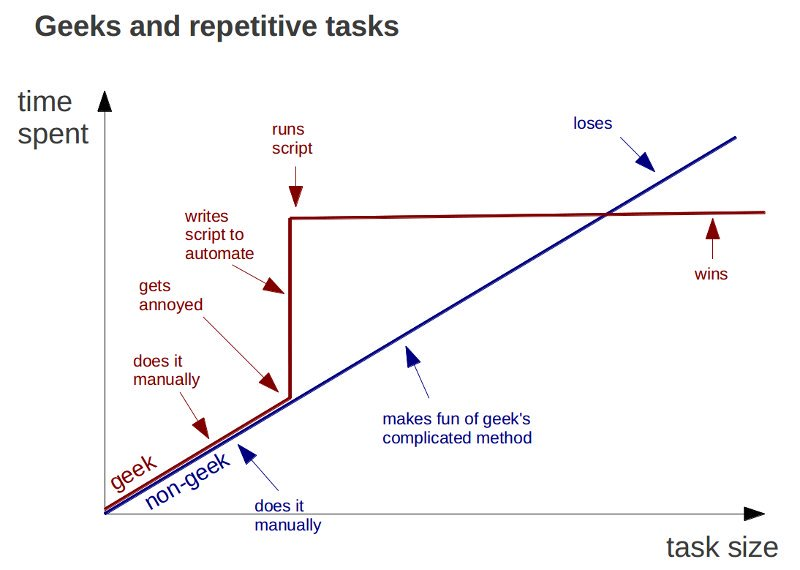
\includegraphics[height=0.7\textheight]{Geeks.jpg}

    \end{itemize}
\end{frame}

\begin{frame}[fragile]
    \begin{itemize}
    \item
    Suppose we find ourselves writing hundreds of repetitive ``pattern instances" like this:

\tiny
\begin{verbatim}
  int plus( int a, int b ) { return (a+b); }
  int minus( int a, int b ) { return (a-b); }
  int times( int a, int b ) { return (a*b); }
  ...
\end{verbatim}
\small

   \pitem
     If we need to write 10 of them - do it in your favourite \alert{programmer's editor} using clone-and-alter.

   \pitem
     What if we need to write 50 of them?  Or 100 of them?  Or 100 int functions and another 100 double functions?

   \pitem
     Are we bored yet?  Is clone-and-alter too error-prone? Then why not..

   \pitem
     Generate such function instances automatically using a
     \alert{shortlived tool},
     scaffolding that you \alert{build} on demand,
     \alert{use} a few times, then \alert{discard}:

   \pitem
     Clearly, all that varies from instance to instance is
     (funcname,operator), eg. \verb!(plus,+)!.

    \pitem
      Specify input format (as a \alert{little language}) and corresponding
      output:

\tiny
\begin{verbatim}
  INPUT:
    each line: F, Op pair
  OUTPUT:
    for each F, Op pair: "int <F>( int a, int b ) { return (a <Op> b); }"
\end{verbatim}
\small

    \end{itemize}
\end{frame}

\subsection{Doing it in Perl - tarball 01.tiny-tool}

\begin{frame}[fragile]
    \begin{itemize}
    \item
      Simple job for a scripting language like \alert{Perl}.

    \pitem
      Here's a Perl oneliner I composed in a minute:

\tiny
\begin{verbatim}
  perl -nle '($f,$op)=split(/,/); print "int ${f}( int a, int b ) { return (a ${op} b); }"' < input
\end{verbatim}
\small

    \pitem
%     What does that do?
%     \begin{itemize}
%      \item
      The basic structure:
\tiny
\begin{verbatim}
  perl -nle 'PERL CODE' < input
\end{verbatim}
\small

     means execute that chunk of Perl code for every line of the input.

      \pitem
      The Perl code:
\tiny
\begin{verbatim}
  ($f,$op)=split(/,/)
\end{verbatim}
\small

     means split the current line on "," into two strings,
     storing the part before the comma into the variable \verb+$f+,
     and the part after the comma into \verb+$op+.

      \pitem
      The Perl code:
\tiny
\begin{verbatim}
  print "int ${f}( int a, int b ) { return (a ${op} b); }"
\end{verbatim}
\small
      means print out the string literal, replacing \verb+${f}+ and \verb+${op}+ with the value of those variables.

%     \end{itemize}


    \pitem
      Don't want to do it in Perl?   (weirdo).
      \pause
      Then use a different tool!

    \pitem
    I wrote it in C in 15 minutes using standard library function
    \alert{strtok()} to split on comma:
    See \alert{01.tiny-tool/genfuncs1.c}.

    \end{itemize}
\end{frame}

\subsection{Improving our Tiny tool - tarball 01.tiny-tool}

\begin{frame}[fragile]
    \begin{itemize}
    \item
      Note that our tool doesn't have to be perfect;
      just good enough to save us time.
 
    \pitem
    Once you have a tiny tool, don't be afraid to modify it:

    \item
    Left-justify the function names in a field of some suitable width:

\tiny
\begin{verbatim}
  perl -nle '($f,$op)=split(/,/); printf "int %-15s( int a, int b ) { return (a${op}b); }\n", $f' < input
\end{verbatim}
\small

    \pitem
    Or, prefix the typename onto function names, eg. \verb+int_plus+:

\tiny
\begin{verbatim}
  perl -nle '($f,$op)=split(/,/); printf "int %-15s( int a, int b ) { return (a${op}b); }\n", "int_${f}"' < input
\end{verbatim}
\small

%   \pitem
%   Noticing all those ``int"s, let's make it easier to change:
%\tiny
%\begin{verbatim}
%  perl -nle '$t="int"; ($f,$op)=split(/,/);
%             printf "${t} %-15s( ${t} a, ${t} b ) { return (a${op}b); }\n", "${t}_${f}"' < input
%\end{verbatim}
%\small

%\item
%    Note the repeated "int"s, we may regard the type 'int' as a parameter,
%    and change our spec to:
%
%\tiny
%\begin{verbatim}
%  INPUT:
%    line 1: typename T eg. int
%    foreach line>1: F, Op pairs
%  OUTPUT:
%    foreach line>1: "T F( T a, T b ) { return (a Op b); }"
%\end{verbatim}
%\small
%
%    \pause
%    \item
%    Modify our Perl code to:
%
%\tiny
%\begin{verbatim}
%  perl -nle 'if($.==1){$t=$_;next} ($f,$op)=split(/,/);...
%             print "${t} ${f}( ${t} a, ${t} b ) { return (a ${op} b); }"'
%\end{verbatim}
%\small

%   \pitem
%   We could let the user set the type within the input, perhaps the first line
%   of input, see \alert{01.tiny-tool/README} for details.

   \pitem
   Why not let the user change the type at any point in the input:

\tiny
\begin{verbatim}
    TYPE,int
    plus,+
    minus,-
    TYPE,double
    plus,+
    minus,-
\end{verbatim}
\small

generates:

\tiny
\begin{verbatim}
    int    int_plus       ( int a, int b ) { return (a+b); }
    int    int_minus      ( int a, int b ) { return (a-b); }
    double double_plus    ( double a, double b ) { return (a+b); }
    double double_minus   ( double a, double b ) { return (a-b); }
\end{verbatim}
\small

    \end{itemize}
\end{frame}



\begin{frame}[fragile]
    \begin{itemize}
\item
To implement this, change the specification to:

\tiny
\begin{verbatim}
  INPUT:
    each line: F, Op pair
  OUTPUT:
    for each F, Op pair:
        if F=="TYPE" then T=Op
        else print "<T> <T>_<F>( <T> a, <T> b ) { return (a <Op> b); }"
\end{verbatim}
\small

\item
Make our Perl one-liner:

\tiny
\begin{verbatim}
  perl -nle '($f,$op)=split(/,/); if( $f eq "TYPE" ) { $t=$op; next; }
             printf "${t} %-15s( ${t} a, ${t} b ) { return (a${op}b); }\n", "${t}_${f}"' < input
\end{verbatim}
\small

%\item
%See \alert{01.tiny-tool/genfuncs3.c} for a C implementation.

\pitem
Final thought, instead of hardcoding the output format in the printf,
we could replace TYPEs with TEMPLATEs in the input, for example:

\tiny
\begin{verbatim}
  TEMPLATE,int int_<0>( int a, int b ) { return (a<1>b); }
  plus,+
  minus,-
  TEMPLATE,double double_<0>( double a, double b ) { return (a<1>b); }
  plus,+
  minus,-
\end{verbatim}
\small

\item
Here, the marker \verb+<0>+ means
"replace this marker with the current value of the first field".
Our Perl one-liner becomes more powerful but shorter:

\tiny
\begin{verbatim}
  perl -nle '@f=split(/,/,$_,2); if( $f[0] eq "TEMPLATE" ) { $t=$f[1]; next; }
             $_=$t; s/<(\d+)>/$f[$1]/g; print' < input
\end{verbatim}
\small

\item
This is now a simple template processor.

    \end{itemize}
\end{frame}

\section{Medium: Generating Prototypes Automatically}

\subsection{proto: (tarball 02.proto)}

\begin{frame}[fragile]
    \begin{itemize}
      \item
      Let's move on to an example medium scale tool I built.

    \item
      While developing C code, you may find certain things
      irritate you.

    \item
      The Pragmatic Programmers describe such things as \alert{broken windows},
      and tell us - in tip 4 - \alert{Don't live with broken windows}.
      Find a way to fix the problem!
  
    \pitem
      One particular thing irritated me some years ago:
      keeping the \alert{prototype declarations} in
      .h files in sync with the \alert{function definitions}
      in the paired .c files that form modules.

    \pitem
      Whenever you \alert{add a public function} to \alert{intlist.c}
      you need to remember to add the corresponding prototype to
      \alert{intlist.h}.

    \pitem
      Even \alert{adding or removing parameters} to existing functions
      means you need to make a corresponding change
      in the prototype too.
      \pause
      What a pain!

    \pitem
      The problem here is that there's a lot of repetition between
      the .c file and the .h file.
      This violates the most important Pragmatic Programmers tip:
      
      \alert{DRY - Don't Repeat Yourself} (tip 11).

    \end{itemize}
\end{frame}

\begin{frame}[fragile]
    \begin{itemize}
    \item
      \alert{Don't live with broken windows} suggests we should find, or
      write, a tool to solve this problem,
      then integrate it into our editor for convenience!

    \pitem
      Years ago, I wrote \alert{proto} to solve this.
      It reads a C file looking for function definitions, and
      produces a prototype (an extern declaration) for each function.

    \pitem
      But this sounds pretty hard.  Don't we need a complete C
      parser?
    \pitem
      I found an easier way.
      I imposed LIMITATIONS on my layout approach to make the tool easier
      to construct: I decided that the
      \alert{whole function heading must be placed on one line}, and
      also that the function heading could
      \alert{only use simple type declarations}
      eg. \verb+typename [**..] paramname+
      (use \alert{typedef} for complex declarations).

    \pitem
      Then I wrote a vi macro bound to an unused key that
      piped the next paragraph into \alert{proto \%} (current filename).
      %Can do same for forward declarations of static functions using \alert{proto -s \%}.
      \pause
      See
      \verb+http://www.doc.ic.ac.uk/~dcw/PSD/article4/+
      for an article I wrote about how easy similar editor extensions
      can be.

    \pitem
     Let's see {\bf proto} in action!

%      \tiny
%\begin{verbatim}
%  http://www.doc.ic.ac.uk/~dcw/PSD/article4/
%\end{verbatim}
%\small

    \end{itemize}
\end{frame}

\section{Large: Reusable ADT modules}
\subsection{hashes, lists, trees, sets etc}

\begin{frame}[fragile]
    \begin{itemize}
    \item
      Most problems are made a lot easier by having a library
      of trusted reusable ADT modules:
      %- whether handwritten or \alert{automatically-generated} (see next topic).
      \begin{itemize}
      \item
      indefinite length \alert{dynamic strings}
      \item
      indefinite length \alert{dynamic arrays}
      %\item
      %indefinite length \alert{sparse dynamic arrays}
      \pause
      \item
      \alert{linked lists} (single or double linked)
      \item
      \alert{stacks} (can just use lists)
      \item
      \alert{queues} and \alert{priority queues}
      \item
      \alert{binary trees}
      \pause
      \item
      \alert{hashes} (aka maps/dictionaries/associative arrays).
      \item
      \alert{sets} of strings - several possible implementations.
      \item
      \alert{bags} - frequency hashes, mapping strings to integers.
      \pause
      \item
      anything else you find useful (.ini file parsers? test frameworks?
      CSV splitters?)
      \end{itemize}
    \pitem
      Unlike C++, the C standard library fails to provide any of the following:
      %(C++ provides the \alert{Standard Template Library}):
      So, either find a collection of such modules that others have
      written, or \alert{build them yourself} as and when you need them, and
      \alert{reuse them} at every opportunity.
    \pitem
      Note: Reuse can be done without OO or generics,
      {\em Make it Easy to Reuse} (PP Tip 12) - just use \verb+void *+.
    \end{itemize}
\end{frame}

\subsection{Some ADTs: tarball 03.adts/example 04.hash-set-eg}

\begin{frame}[fragile]
    \begin{itemize}
    \item
     To get you started, {\bf tarball 03.adts} includes a group
     of half a dozen ADTs (plus unit test programs) that I've written over
     the years,
     plus a Makefile to package them as the \alert{libADTs.a} library.

    \pitem
      Investigate them all at your own leisure - but \alert{make install}
      them now so
      they're installed in your TOOLDIR (\verb+~/c-tools+) directory.

    \pitem
      Next, {\bf tarball 04.hash-set.eg} contains an example application
      that uses some of those ADTs, specifically:

      \begin{itemize}
      \pitem
        \alert{Hashes} - \alert{(key,value)} storage implemented using hash
	tables, where the keys are strings, and the values are generic
	\alert{void *} pointers - yes, it's our old friend hash.c, after
	Lecture 2's memory-leak fixes and profiling-led optimizations.

      \pitem
        and \alert{Sets of strings}.

      \pitem
        Then combines them to represent family information, i.e.
        a mapping from a \alert{named parent} to \alert{set of named children}.

      \item
        It's left for you to examine and play with.

      \end{itemize}
      
      \pitem
        \alert{C+hashes+sets} makes it easy to pretend that you're programming
	in Perl:-)
    \end{itemize}
\end{frame}

\section{Large: Autogenerating ADTs}
\subsection{datadec (tarball 06.datadec/07.datadec-eg)}

\begin{frame}[fragile]
    \begin{itemize}
    \item
      \alert{Principle:}
      It's often an excellent idea to
      \alert{import cool features from other languages}.
    %\item
    %  For example, Perl teaches us the importance of
    %  \alert{hashes}
    %  (aka Java dictionaries).
    %  %- \alert{(key,value)} storage implemented using hash tables.
    %  We've already seen a hash module do this in C.
    \pitem
      Many years ago, I realised that one of the best
      features of \alert{functional programming languages}
      such as Haskell is the ability to define
      \alert{inductive data types}, as in:
\begin{verbatim}
intlist = nil or cons( int head, intlist tail );
\end{verbatim}
    \pitem
      I'd dearly love to have that ability in C.

    \pitem
      If only there
      was a tool that \alert{reads such type definitions} and automatically
      writes a \alert{C module that implements them}..
    \pitem
      I looked around, {\em but I couldn't find one}.
      Noone seemed to have ever suggested that such a tool could
      be useful!
    \pitem
      Decision time: do I abandon my brilliant idea, or \alert{build the tool}?
    \pitem
      Cost/benefit analysis: a serious tool, a mini-compiler (with parser, lexical analyser,
      data structures, tree walking code generator):
      at least a week's work!  Think hard!
    \end{itemize}
\end{frame}

\begin{frame}[fragile]
    \begin{itemize}
    \item
      I built the tool!  After a fortnight's work, the
      result was \alert{datadec} - in the \alert{06.datadec} directory
      (also installed throughout DoC labs).
      After installing it, use as follows:
    \pitem
      In \alert{07.datadec-eg} you'll find an input file
      \alert{types.in} containing:
      \small
\begin{verbatim}
TYPE {
       intlist =  nil or cons( int head, intlist tail );
       tree    =  leaf( string name )
               or node( tree left, tree right );
}
\end{verbatim}
    \pitem
       To generate a C module called \alert{datatypes} from \alert{types.in},
       invoke:
\begin{verbatim}
  datadec datatypes types.in
\end{verbatim}
    \pitem
       This creates \alert{datatypes.c} and \alert{datatypes.h}, two
       normal looking C files,
       you can read them, write test programs against the interface,
       use them in production code with no license restrictions.
       \pause
       But don't modify these files - if you do then you can't...
    \pitem
       ... change \alert{types.in} later - suppose you realise that
       a tree node also needs to store a name (just as the leaves do).
       Change the type defn, rerun \alert{datadec}.  The \verb+tree_node()+
       constructor now takes 3 arguments!
    \end{itemize}
\end{frame}

\begin{frame}[fragile]
    \begin{itemize}
    \item
      Let's look inside \alert{datatypes.h},
      to find what \alert{tree} functions \alert{datadec} generates, and how to
      use them.
    \pitem
      There are two \alert{constructor functions}, one for each {\em shape of tree}:
%\tiny
\begin{verbatim}
  extern tree tree_leaf( string name );
  extern tree tree_node( tree l, tree r );
\end{verbatim}
%\small

    \pitem
      So, this allows us to build trees as in:
%\tiny
\begin{verbatim}
  tree t1 = tree_leaf( "absolutely" );
  tree t2 = tree_leaf( "fabulous" );
  tree t = tree_node( t1, t2 );
\end{verbatim}
%\small

    \pitem
      Then a function telling you \alert{which shape a tree is}:
      is it a leaf or a node?
%      \tiny
\begin{verbatim}
  typedef enum { tree_is_leaf, tree_is_node } kind_of_tree;
  extern kind_of_tree tree_kind( tree t );
\end{verbatim}
%      \small

    \pitem
      Then two \alert{deconstructor functions} which, given a tree of the
      appropriate shape, breaks it into it's constituent pieces:
%      \tiny
\begin{verbatim}
  extern void get_tree_leaf( tree t, string *namep );
  extern void get_tree_node( tree t, tree *lp, tree *rp );
\end{verbatim}
%      \small
\end{itemize}

\end{frame}


\begin{frame}[fragile]
    \begin{itemize}
    \item
     These allow you to write \alert{tree-walking} code like this leaf-counter:
%\tiny
\small
\begin{verbatim}
int nleaves( tree t )
{
    if( tree_kind(t) == tree_is_leaf )
    {
        string name; get_tree_leaf( t, &name );
        return 1;             // leaf( name ): contains 1 leaf.
    } else
    {
        tree l, r; get_tree_node( t, &l, &r );
        // node( l, r ): process l and r trees.
        return nleaves(l) + nleaves(r);
    }
}
\end{verbatim}
\small

   \item
 In Haskell, this'd be:
%\tiny
\begin{verbatim}
 nleaves(leaf(name)) = 1
 nleaves(node(l,r))  = nleaves(l) + nleaves(r)
\end{verbatim}
%\small

\end{itemize}
\end{frame}


\begin{frame}[fragile]
    \begin{itemize}
    \item
      The final function prints a tree to a writable file handle, in human
      readable format:
      %(you can control the format - \verb+man datadec+ for details):
%      \tiny
\begin{verbatim}
  extern void print_tree( FILE *out, tree t );
\end{verbatim}
%      \small
    \pitem
     To see all the above in use, see \verb+mintesttree.c+.

    \pitem
      By default, \alert{datadec} does not generate free functions.  Why?
      \pause
      Hard to do right due to shallow vs deep considerations.

%    \pitem
%      However: you can now run \alert{datadec -f..} to get experimental
%      \alert{free\_TYPE()} functions,
%      If you don't want a parameter freed, mark it in the input file with a `-',
%      as in:
%
%      \tiny
%\begin{verbatim}
%  tree  =  leaf( -string name )
%        or node( tree left, tree right );
%\end{verbatim}
%\small

    %\pitem

    \pitem
      You can now run \alert{datadec -f..} to get experimental
      \alert{free\_TYPE()} functions,
      although you still have to be careful using these -
      see the README file for details.

%     If you use \alert{datadec -f} and do free any "string" parameters,
%     you may need to define how to free a string, by adding the following
%     section to your types.in:
%
%      \tiny
%\begin{verbatim}
%  GLOBAL {
%  #define free_string(s) free(s)
%  }
%\end{verbatim}
%\small

    \pitem
     Looking back, I now view the \alert{fortnight} I spent building datadec
     (and, more recently, the day or two adding \alert{free\_TYPE()} support)
     as the \alert{single best investment of programming time} in my career.
     I have saved \alert{hundreds of days} programming time using it -
     \alert{and so can you!}

    \pitem
    You can read a 3-part article I wrote about how I designed datadec here:

%     \tiny
\begin{verbatim}
  http://www.doc.ic.ac.uk/~dcw/PSD/article8/
\end{verbatim}
%\small

\end{itemize}
\end{frame}

%\begin{frame}[plain]
\begin{frame}
Remember:

%\centering
\begin{center}
%  \vspace{10pt}
  
\includegraphics[height=0.8\textheight]{Build.png}
\end{center}

(and learn Perl, it's great!)

\end{frame}

\end{document}
